\documentclass[10pt,a4paper]{article}
\usepackage[margin=23mm]{geometry}
\usepackage[T1]{fontenc}
\usepackage{mathpazo,microtype,amsmath,amssymb,booktabs,tabularx,xcolor,tikz,sectsty}
\usepackage[colorlinks=true,linkcolor=blue!55!black,urlcolor=blue!55!black,citecolor=blue!55!black]{hyperref}
\usepackage{xurl}
\hypersetup{pdftitle={GlobalStack: Scoped Local Azure Emulation with Executable Cross-Service Checks},pdfsubject={Scoped technical draft; authorship pending}}
\usetikzlibrary{positioning,arrows.meta}
\definecolor{ink}{HTML}{17577B}
\definecolor{good}{HTML}{20836B}
\definecolor{control}{HTML}{C47728}
\allsectionsfont{\color{ink}}
\setlength{\parskip}{4pt}
\setlength{\parindent}{0pt}
\newcommand{\SnapshotDate}{2026-11-04}
\newcommand{\NativeCount}{9}
\newcommand{\EpisodeCount}{8}
\newcommand{\ProviderOperationCount}{50}
\newcommand{\LocalPassed}{559}
\newcommand{\LocalSkipped}{1}
\newcommand{\RepositoryPassed}{19}

\title{\color{ink}GlobalStack: Scoped Local Azure Emulation\protect\\with Executable Cross-Service Checks}
\author{}
\date{Technical draft. Author information pending.\\Validation snapshot: \SnapshotDate}
\begin{document}
\maketitle
\begin{abstract}
A successful infrastructure deployment does not establish that application events reach their intended destination. GlobalStack combines a local Azure management surface, selected service runtimes, and native infrastructure-as-code runners to make this distinction executable. We report a bounded preview evaluation: \NativeCount{} native platform configurations with one sample each, three pinned Microsoft Quickstart templates, and two first-party cross-service scenarios. Each new scenario tests a connected configuration, two broken configurations, recovery, and resource cleanup through real loopback HTTP. All \EpisodeCount{} episodes satisfy their specified test expectations. Of the four deliberately broken configurations, three still report workflow success while failing the intended application outcome. These are constructed controls, not an estimate of failures in Azure or user deployments. The work exposed and corrected literal-value coercion and incomplete runtime cleanup. We release the test inputs, results, toolchain recipes, and explicit support boundaries. No live Azure comparison was performed in this validation; the results establish execution of the selected local paths rather than general Azure equivalence.
\end{abstract}

\section{Problem and scope}
Infrastructure-as-code (IaC) tools describe resources and their relationships, but successful creation is only one requirement of an application. A workflow can reference an existing but incorrect secret. A publisher can accept an event after its subscription is deleted. Both conditions can leave resources readable and operations apparently successful while the business outcome is absent or incorrect.

GlobalStack is a local development system for exercising selected Azure deployments and service interactions. Its public preview is intended for trusted workloads on isolated development hosts. The contribution described here is an executable validation method and its implementation: native provisioning, observable HTTP service interactions, deliberate wiring faults, restoration, and cleanup. This paper does not introduce a new model benchmark, report model-generated deployments, or claim complete Azure emulation.

We ask three bounded questions. First, can the selected native clients provision, inspect, and remove their reference samples? Second, can local service interactions produce an exact expected application result? Third, can tests distinguish a successful operation from an incorrectly wired application and detect residual runtime state after deletion? These questions are answered over a declared set of fixtures. They do not define a denominator for all Azure behavior.

\section{System design}
\subsection{Management and service state}
The management server exposes supported resource and deployment routes over HTTP. A resource store represents management records. Resource creation and deletion invoke runtime synchronization hooks, which connect those records to service-specific state. Selected data-plane routers expose executable operations, including Key Vault secret reads and Event Grid publication and webhook delivery. A local workflow runner evaluates supported expressions and performs supported actions.

This separation matters for correctness. A management record can be correct while a runtime endpoint still serves stale state. Conversely, a valid deployment can connect the wrong runtime resources. The validation therefore reads management resources, exercises service endpoints, and verifies cleanup across both surfaces.

\begin{figure}[ht]
\centering
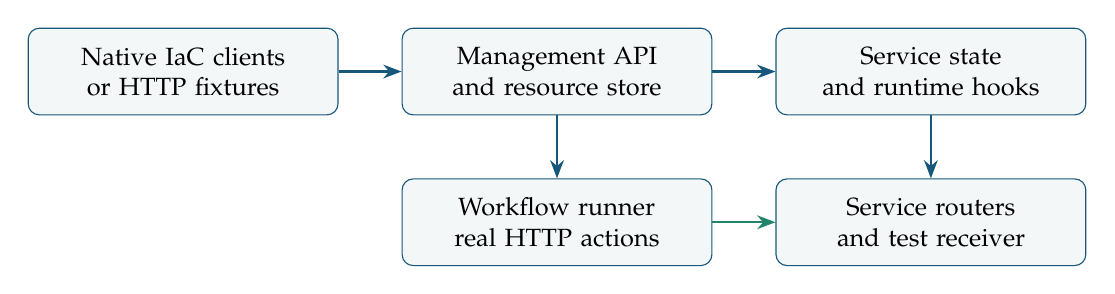
\begin{tikzpicture}[node distance=8mm,box/.style={draw=ink,rounded corners,align=center,text width=37mm,minimum height=11mm,fill=ink!5,font=\small},>={Stealth}]
\node[box] (client) {Native IaC clients\\or HTTP fixtures};
\node[box,right=of client] (arm) {Management API\\and resource store};
\node[box,right=of arm] (runtime) {Service state\\and runtime hooks};
\node[box,below=of arm] (workflow) {Workflow runner\\real HTTP actions};
\node[box,below=of runtime] (receiver) {Service routers\\and test receiver};
\draw[->,thick,ink] (client)--(arm);
\draw[->,thick,ink] (arm)--(runtime);
\draw[->,thick,ink] (arm)--(workflow);
\draw[->,thick,good] (workflow)--(receiver);
\draw[->,thick,ink] (runtime)--(receiver);
\end{tikzpicture}
\caption{The evaluated local architecture. The test receiver is a small HTTP application, not an emulated Azure Functions deployment. Service support is operation-specific.}
\end{figure}

\subsection{Native runners}
The native matrix includes Terraform and OpenTofu using AzAPI, Pulumi TypeScript, Python and YAML using Azure Native, Ansible, Azure CLI REST, Bicep, and ARM JSON. Generated runner contexts separate tool execution from endpoint routing. The harness selects the local provider and supplies a development identity. This identity supports the local protocol path; it does not reproduce Azure tenant isolation or RBAC enforcement.

Each sample runs build, lint, unit tests, deploy, provider lifecycle, integration tests, and destroy. The meaning of a stage depends on the platform. In particular, the integration stage in the native reference samples does not by itself establish an application event path. The separate cross-service experiments below supply that evidence. Terraform results concern AzAPI, not the AzureRM provider.

\subsection{Support boundaries}
Registered resource types, accepted management operations, executable service behavior, and live-cloud conformance are distinct levels of evidence. GlobalStack's service scope and conformance documents distinguish these levels. A registration count cannot measure fidelity. The broader historical 30-service validator still depends on missing artifacts and optional backend matrices and is not reported as passing in this snapshot.

The tested state is ephemeral. Unsupported paths and invalid inputs have selected rejection tests, but this paper makes no universal fail-closed claim. Workflow expression coverage is partial. Retry policy, delivery ordering, eventual delivery, sustained throughput, durable recovery, and multi-tenant isolation are not established by these experiments.

\section{Validation method}
\subsection{Fixtures and provenance}
We use three fixture groups. The native group contains one first-party sample per platform. These are smoke configurations, not nine independent application architectures. The upstream group contains three unmodified Microsoft Azure Quickstart templates: Storage account creation, Key Vault creation, and Event Grid \cite{quickstarts}. Their original bytes, source revision, SHA-256 digests, and MIT license are retained. The Storage example checks management behavior. Key Vault adds a secret read over HTTP. Event Grid adds publication and exact webhook checks with broken-routing and restoration controls.

The third group contains two new first-party scenarios. Their inputs and outcome checks are maintained in the same repository as the emulator. This enables regression testing but creates an oracle-bias risk. Neither first-party fixtures nor unmodified upstream templates establish live Azure equivalence on their own.

\subsection{Two cross-service scenarios}
\textbf{Configuration enrichment.} A Logic Apps workflow reads a configuration value from Key Vault and posts an enriched course record to an HTTP receiver. The intended result contains the request identifier, course identifier, and the expected office value. One control changes the workflow to read an existing secret containing the wrong office. A second control references a missing secret. Restoring the original reference must restore the exact result.

\textbf{Event routing.} A Logic Apps workflow transforms a course record into an Event Grid event and publishes it to a topic. A scoped subscription delivers the event to the intended receiver. One control deletes the subscription. A second recreates it with the wrong destination. Restoring the intended destination must restore delivery. The input includes a unique request identifier and timestamp, and the expected event includes the exact identifier, subject, event type, timestamp, data version, and data object.

Both scenarios create resources using the management API and check successful deployment and resource read-back. The workflow uses its default HTTP transport. Test-owned loopback ports map incoming requests to fixed Azure hostnames at the router boundary; no service response or workflow transport is mocked. This routing adaptation is part of the local harness and is not evidence about Azure DNS, TLS, or authentication behavior.

\subsection{Outcome and control predicates}
For an invocation $i$, let $r_i$ be its unique identifier, $d_i$ its intended receiver path, and $p_i$ its expected JSON payload. Let $R_i$ be the sequence of deliveries observed during that invocation with the same identifier. Retain repeated deliveries as separate observations and define the filtered sequence
\begin{align}
A_i &= [x\in R_i : \operatorname{path}(x)=d_i],\\
O_i &= (|A_i|=1)\ \land\ (\operatorname{body}(A_i[1])=p_i).
\end{align}
The second term is evaluated only when the first is true. JSON equality here is structural and type-sensitive. An event at the wrong path, a missing event, a duplicate at the intended path, or a wrong field fails $O_i$. Exactly one delivery means one observed delivery in the local test interval; it is not an exactly-once delivery guarantee for a distributed service.

We separately record deployment acceptance $D_i$, observed service-boundary HTTP traffic $H_i$, and workflow success $W_i$. A positive episode requires $D_i\land H_i\land W_i\land O_i$. A deliberately broken episode requires $D_i\land H_i\land\neg O_i$ plus its specific expected status or destination observation. Thus a control passes the test when it demonstrates the intended failure. The harness does not relabel a broken application as a working deployment.

For each scenario, cleanup $C$ requires successful group deletion, management reads returning 404 for the group and workflow, and a request to the deleted service's data-plane endpoint returning 404. A complete scenario must satisfy the four episode expectations and $C$. This checks the addressed resources, not the absence of every possible process, cache, or background task.

\subsection{Execution and reproducibility}
The snapshot uses Linux x86\_64, four logical CPUs, and approximately 31 GiB of RAM. Native jobs run in three isolated checkout groups. A disk guard stops work before the required 40 GiB free-space reserve is crossed. These are observed host characteristics, not minimum hardware requirements. No live Azure deployment or paid model request is part of this validation.

Pinned versions cover the principal CLI tools and direct sample SDK dependencies. The TypeScript sample uses an npm lockfile and \texttt{npm ci}; the root workspace also has a lockfile. The native run uses one standalone Terraform base and four derived validation images to share layers. Their recipes and observed image identifiers are retained. We have not built every standalone runner Dockerfile in this experiment. Mutable base tags, operating-system packages, upstream installation scripts, and unpinned Python transitive dependencies remain. The artifact supports rerunning the declared checks, not a byte-identical image rebuild claim.

\section{Results}
\subsection{Native and local checks}
Table~\ref{tab:matrix} reports the current native matrix. Each row is one sample and all seven stages are required, including destruction. The provider-lifecycle reports contain \ProviderOperationCount{} operation checks across the nine runs. These include overlapping checks and are not a count of distinct Azure APIs.

\begin{table}[ht]
\centering\small
\caption{Native smoke matrix. Each row has one sample.}\label{tab:matrix}
\begin{tabular}{lll}\toprule
Configuration & Native tool or SDK & Result \\\midrule
Ansible & Core 2.21.6; collection 3.21.0 & 7/7; cleanup passed \\
ARM JSON & Azure CLI 2.92.0 & 7/7; cleanup passed \\
Bicep & Bicep 0.48.1; Azure CLI 2.92.0 & 7/7; cleanup passed \\
Azure CLI REST & Azure CLI 2.92.0 & 7/7; cleanup passed \\
OpenTofu HCL & OpenTofu 1.13.2; AzAPI 2.13.0 & 7/7; cleanup passed \\
Pulumi Python & CLI 3.273.0; Azure Native 3.30.0 & 7/7; cleanup passed \\
Pulumi TypeScript & CLI 3.273.0; Azure Native 2.92.3 & 7/7; cleanup passed \\
Pulumi YAML & CLI 3.273.0; Azure Native 3.18.0 & 7/7; cleanup passed \\
Terraform HCL & Terraform 1.17.1; AzAPI 2.13.0 & 7/7; cleanup passed \\
\bottomrule\end{tabular}

\end{table}

The local conformance command reports \LocalPassed{} passing tests and \LocalSkipped{} explicitly opt-in Docker-dependent Kubernetes test skipped. Repository policy tests report \RepositoryPassed{} passes. Three upstream template tests are included in the local suite. Separately executed Key Vault, Event Grid, and Logic Apps packs report 99, 45, and 62 cases respectively. These suites overlap and must not be added to form an Azure-coverage score. The archived preview-2 result is an earlier snapshot with 556 local passes; this draft's record identifies the new runtime and evidence revisions explicitly.

\subsection{Cross-service observations}
Table~\ref{tab:flows} contains all eight newly recorded episodes. Both connected and restored episodes in each scenario produce the exact expected payload. All four deliberately broken configurations fail the application outcome assertion as intended. Three of these four still report workflow success. This demonstrates a specific limitation of using operation success as the only local wiring check. It is not a measured prevalence of such failures in real deployments.

\begin{table}[ht]
\centering\small
\caption{Constructed controls and positive episodes. ``No'' in the outcome column is expected for the broken configurations.}\label{tab:flows}
\begin{tabular}{llll}\toprule
Scenario & Configuration & Workflow & Exact outcome \\\midrule
Enrichment & connected & Succeeded & Yes \\
Enrichment & wrong-config-reference & Succeeded & No (expected) \\
Enrichment & missing-config-reference & Failed & No (expected) \\
Enrichment & restored & Succeeded & Yes \\
Event routing & connected & Succeeded & Yes \\
Event routing & deleted-subscription & Succeeded & No (expected) \\
Event routing & wrong-destination & Succeeded & No (expected) \\
Event routing & restored & Succeeded & Yes \\
\bottomrule\end{tabular}

\end{table}

\begin{figure}[ht]
\centering
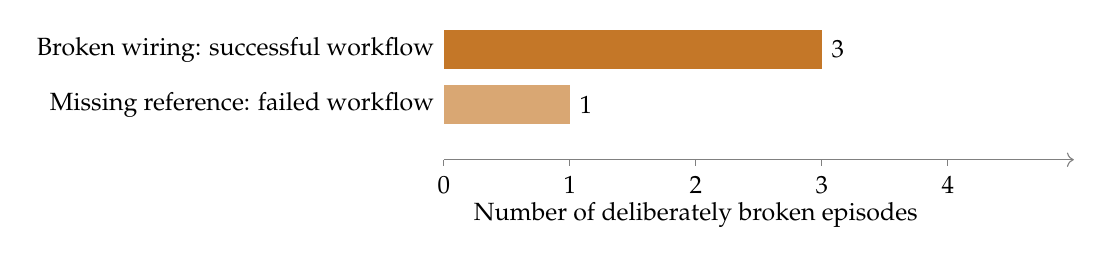
\begin{tikzpicture}[x=16mm,y=7mm,font=\small]
\draw[->,gray] (0,0)--(5,0);
\foreach \x in {0,...,4} {\draw[gray] (\x,0)--(\x,-.12) node[below,text=black]{\x};}
\node[anchor=east] at (0,1) {Missing reference: failed workflow};
\node[anchor=east] at (0,2) {Broken wiring: successful workflow};
\fill[control!65] (0,.65) rectangle (1,1.35);
\fill[control] (0,1.65) rectangle (3,2.35);
\node[anchor=west] at (1,1) {1};\node[anchor=west] at (3,2) {3};
\node[anchor=north] at (2,-.6) {Number of deliberately broken episodes};
\end{tikzpicture}
\caption{Workflow status within four constructed negative controls. All four failed the intended outcome. The count is a property of the test design, not an accuracy or prevalence estimate.}
\end{figure}

Both scenario cleanup checks pass. The evidence records the unique input, service-boundary status, receiver path and payload, workflow status, assertion result, and cleanup result. The test report is generated only after all assertions succeed. Failed test processes must be retained separately; absence of a report is not a passing result.

\subsection{Defects found through executable checks}
\textbf{Literal-value coercion.} The workflow evaluator previously converted numeric-looking JSON strings into numbers outside expression argument parsing. An Event Grid event with the literal data version \texttt{"1.0"} reached the service as a number and failed its schema check. The correction preserves literal JSON types while parsing numeric constants inside supported expression arguments. A regression test also covers leading-zero strings, quoted literal text, numbers, booleans, arrays, and existing supported arithmetic. The Azure expression reference distinguishes expressions from literal values \cite{expressions}; this fix is not a claim to implement the full expression language.

\textbf{Management deletion without runtime deletion.} Resource-group deletion previously removed management records without invoking deletion hooks for the resources in that group. A Key Vault secret remained readable after its group disappeared. The correction enumerates the group's resources, invokes the runtime deletion hooks in child-first order, and is checked by the new post-delete data-plane assertions. The selected regression establishes cleanup for these flows; other runtime backends require their own checks.

These findings illustrate why read-back, live requests, and cleanup are separate obligations. The repaired code is evaluated on the same authored scenarios, so these findings should be interpreted as engineering regressions rather than an independent comparative study.

\section{Related systems and API drift}
Microsoft's Azurite supports local Blob, Queue, and Table development and documents differences from Azure Storage \cite{azurite}. Microsoft's Service Bus emulator provides local messaging behavior with explicit protocol and persistence limitations \cite{servicebus}. These projects demonstrate the value of a declared support boundary for local development. We have not run a comparative evaluation against them and do not infer relative completeness, performance, or fidelity.

Microsoft's Azure REST API specifications provide a versioned source for reviewing API changes \cite{specs}. GlobalStack includes a weekly specification watcher and an opt-in differential harness with selected AKS status and error cases. A changed specification is a review signal, not proof of a changed runtime behavior. Conversely, unchanged documentation does not prove unchanged service behavior. This draft reports no new live differential results.

A future live comparison should run the same versioned scenario against Azure and the local system, retaining request shape, normalized responses, observable side effects, event correlation, and cleanup outcomes. Normalization must be explicit and limited to genuinely variable fields. API version, region, test time, account constraints, and known deviations should accompany every record. Costs and credentials require a separately approved live run. This protocol remains future work for the cross-service scenarios described here.

\section{Limitations and release interpretation}
\textbf{Selection and oracle bias.} One sample per platform exercises a narrow configuration. The two new flows share the workflow engine and are first-party fixtures, so their success is not independent external validation. Upstream templates reduce authorship coupling but do not supply live-cloud outcome traces. There is no randomly sampled workload corpus, held-out evaluation, or baseline comparison.

\textbf{Local execution model.} The tested event paths complete synchronously through loopback HTTP. No retry, timeout distribution, load, network partition, or eventual consistency experiment is reported. Hostname adaptation and development identity are harness facilities. The receiver is a test application rather than a deployed Azure compute service.

\textbf{Security and privacy.} The preview is not a production security boundary. Security CI includes dependency auditing, secret scanning, and full-tree JavaScript CodeQL analysis. The previous preview's security correction and remaining reviewed findings are recorded separately in the repository. Passing these checks does not establish absence of vulnerabilities, compliance certification, complete capture sanitization, or suitability for untrusted tenants. Evidence in this draft uses synthetic local identifiers and test values.

\textbf{Reproduction and provenance.} Version pins improve stability but do not freeze the complete software supply chain. Results apply to the tested source revision and retained inputs. Revisions are included in the artifact record for reproducibility, not as evidence of correctness. The current paper is a technical draft with author information pending and has not been submitted to arXiv.

\section{Conclusion}
The scoped preview executes nine native reference configurations and two explicit multi-service workflows, alongside pinned upstream template checks. Broken-wiring controls demonstrate that operation success can coexist with a failed application outcome. Live HTTP assertions and post-delete checks uncovered two concrete implementation defects. The resulting artifact is useful for reproducing these local paths and extending their tests. Broader Azure equivalence requires additional independently authored scenarios and measured live differential validation.

\appendix
\section{Artifact and reproduction record}
Source: \url{https://github.com/divine-ai-com/globalstack}. The draft, evidence, and shared-image recipes are in \path{docs/research/globalstack/}. The historical source preview is \texttt{v0.1.0-preview.2}; this draft includes subsequent changes and does not silently replace that tag's results.

\small
Base runtime and native matrix revision: \texttt{0f9071b993d3}.

TypeScript dependency rerun revision: \texttt{0f523fd77add}.

Flow evidence revision: \texttt{0f9071b993d3}.

Full revisions, image identifiers, commands, and limitations are retained in the adjacent JSON records.

Minimum free disk during the native runs: 103.25 GiB.

\normalsize

\begin{thebibliography}{9}
\bibitem{quickstarts} Microsoft Azure. Azure Quickstart Templates. Pinned fixture revision and file digests are retained in the artifact. \url{https://github.com/Azure/azure-quickstart-templates}.
\bibitem{expressions} Microsoft. Reference guide to functions in expressions for Azure Logic Apps and Power Automate. \url{https://learn.microsoft.com/en-us/azure/logic-apps/expression-functions-reference}. Accessed November 2026.
\bibitem{azurite} Microsoft. Use the Azurite emulator for local Azure Storage development. \url{https://learn.microsoft.com/en-us/azure/storage/common/storage-use-azurite}. Accessed November 2026.
\bibitem{servicebus} Microsoft. Overview of the Azure Service Bus emulator. \url{https://learn.microsoft.com/en-us/azure/service-bus-messaging/overview-emulator}. Accessed November 2026.
\bibitem{specs} Microsoft Azure. Azure REST API specifications. \url{https://github.com/Azure/azure-rest-api-specs}. Accessed November 2026.
\end{thebibliography}
\end{document}
